% Created 2022-02-12 Sat 22:08
\documentclass[9pt, b5paper]{article}
\usepackage{xeCJK}
\usepackage{minted}
\usepackage{xltxtra}
\usepackage{bera}
\usepackage[T1]{fontenc}
\usepackage[scaled]{beraserif}
\usepackage[scaled]{berasans}
\usepackage[scaled]{beramono}
\usepackage{xcolor}
\usepackage{multirow}
\usepackage{multicol}
\usepackage{float}
\usepackage{textcomp}
\usepackage{algorithm}
\usepackage{algorithmic}
\usepackage{latexsym}
\usepackage{natbib}
\usepackage{geometry}
\geometry{left=1.2cm,right=1.2cm,top=1.5cm,bottom=1.2cm}
\newminted{common-lisp}{fontsize= criptsize} 
\usepackage[xetex,colorlinks=true,CJKbookmarks=true,linkcolor=blue,urlcolor=blue,menucolor=blue]{hyperref}
\author{deepwaterooo}
\date{\today}
\title{Android Jetpack MVVM app coding practice}
\hypersetup{
  pdfkeywords={},
  pdfsubject={},
  pdfcreator={Emacs 27.1 (Org mode 8.2.7c)}}
\begin{document}

\maketitle
\tableofcontents


\section{Android Jetpack MVVM app coding practice}
\label{sec-1}
\begin{itemize}
\item 这是上一个项目所参考过的项目(主要是设计与封装),相对更为完整一点儿,因为涉及到更多的
MVVM的架构设计、封装与应用,原本只想读一下原作者的源码,理解代码就可以了完
事儿了。但是考虑到上次照猫画虎的过程中所出现过的种种bug以及fix的过程,还是觉得练习的过程也比较重要,所
以在拿自己现有的代码,把原人的设计、原理以及源码都再在自己的环境中重
新构建一遍,修改自己构建过程中所出现过的问题
\begin{itemize}
\item databinding的部分,因为reference导入的问题,还是浪费了几个小时的时
间才pass掉databinding BR类找不到的问题:这个更像是成了一块心病了:几个月前最开始学
习databinding的时候是layout binding类怎么也生成不出来,因为layout里有错。。。
现在是数据库beans类、model类reference有错导致BR生成不出来。。。)
以后要记错:databinding过程中所有的错,都终将追逆到或是layout中的
错,或是代码中的错,把这些都fix掉之后,一般那些binding类还是会自动
就出来的。这个还是要相对再多练习一些
\item R.id.design$_{\text{bottom}}$$_{\text{sheet的小问题很容易解决}}$
\item 地图没能显示出来,这个,改天如果对地图有需求的时候会再看看
\item 这一两个项目过程中一路走过的弯路,都是自己专业成长里必经之路,且错且珍惜呵呵
\item 这个项目最后放手的点在:项目中使用了中国的高德地图的api,需要注
册账号,导致最终没有注册的情况下很多功能就出不来了。我对自己注册一
个账户/md5匹配、链接api有信心,但我不想再浪费更多的精力在一个中国
地图、我完全用不着的地图上。。。如果是美国加州湾区地图,我可能还有兴趣写个自己的地图代替
GPS,但再好的项目,运行到这里,达到了自己练习的目的,我认为也是该结束了
\item 会再稍微去参考一下新添加的记事本功能,但这个仓库可能就不再更新了
\end{itemize}
\end{itemize}

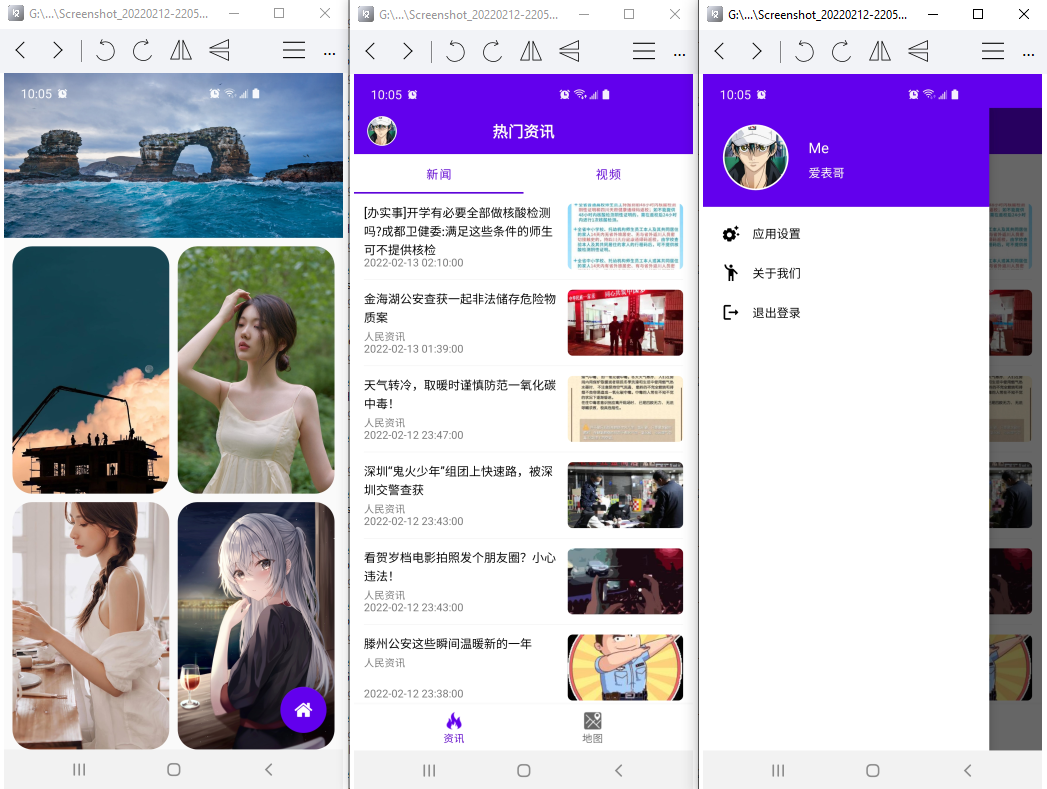
\includegraphics[width=.9\linewidth]{./pic/screens2.png}

\begin{itemize}
\item 接下来会找更适合自己的安卓项目学习,多抓一些项目练习,以及拓展相关的知识面
\end{itemize}
% Emacs 27.1 (Org mode 8.2.7c)
\end{document}